\documentclass[12pt]{article}
\usepackage[a4paper,margin=1in]{geometry}
\usepackage{amsmath,amssymb}
\usepackage{graphicx}
\usepackage{siunitx}
\sisetup{per-mode=symbol}
\usepackage{gvv}

\title{Matrix 1.11.2}
\author{ai25btech11015 -- M Sai Rithik}
\date{}

\begin{document}
\maketitle

\section*{Question}
Find the unit vector along $\Vec{PQ}$, where $P=(2,1,-1)$ and $Q=(4,4,-7)$.  


\section*{Solution}

\subsection*{Step 1: Vector $\Vec{PQ}$}
The given points are
\[
P = \myvec{2 \\ 1 \\ -1}, 
\quad Q = \myvec{4 \\ 4 \\ -7}.
\]
Hence,
\begin{equation}
\Vec{PQ} = Q - P = \myvec{4 \\ 4 \\ -7} - \myvec{2 \\ 1 \\ -1}
= \myvec{2 \\ 3 \\ -6}.
\end{equation}

\subsection*{Step 2: Magnitude of $\Vec{PQ}$}
\begin{equation}
\|\Vec{PQ}\| = \sqrt{2^2 + 3^2 + (-6)^2}
= \sqrt{4+9+36}
= \sqrt{49} = 7.
\end{equation}

\subsection*{Step 3: Unit vector along $\Vec{PQ}$}
The unit vector is
\begin{equation}
\Vec{OA} = \frac{\Vec{PQ}}{\|\Vec{PQ}\|}
= \frac{1}{7}\myvec{2 \\ 3 \\ -6}.
\end{equation}

\section*{Final Answer}
\[
\boxed{\Vec{OA} = \frac{1}{7}\myvec{2 \\ 3 \\ -6}}
\]

\begin{figure}[h!]
    \centering
    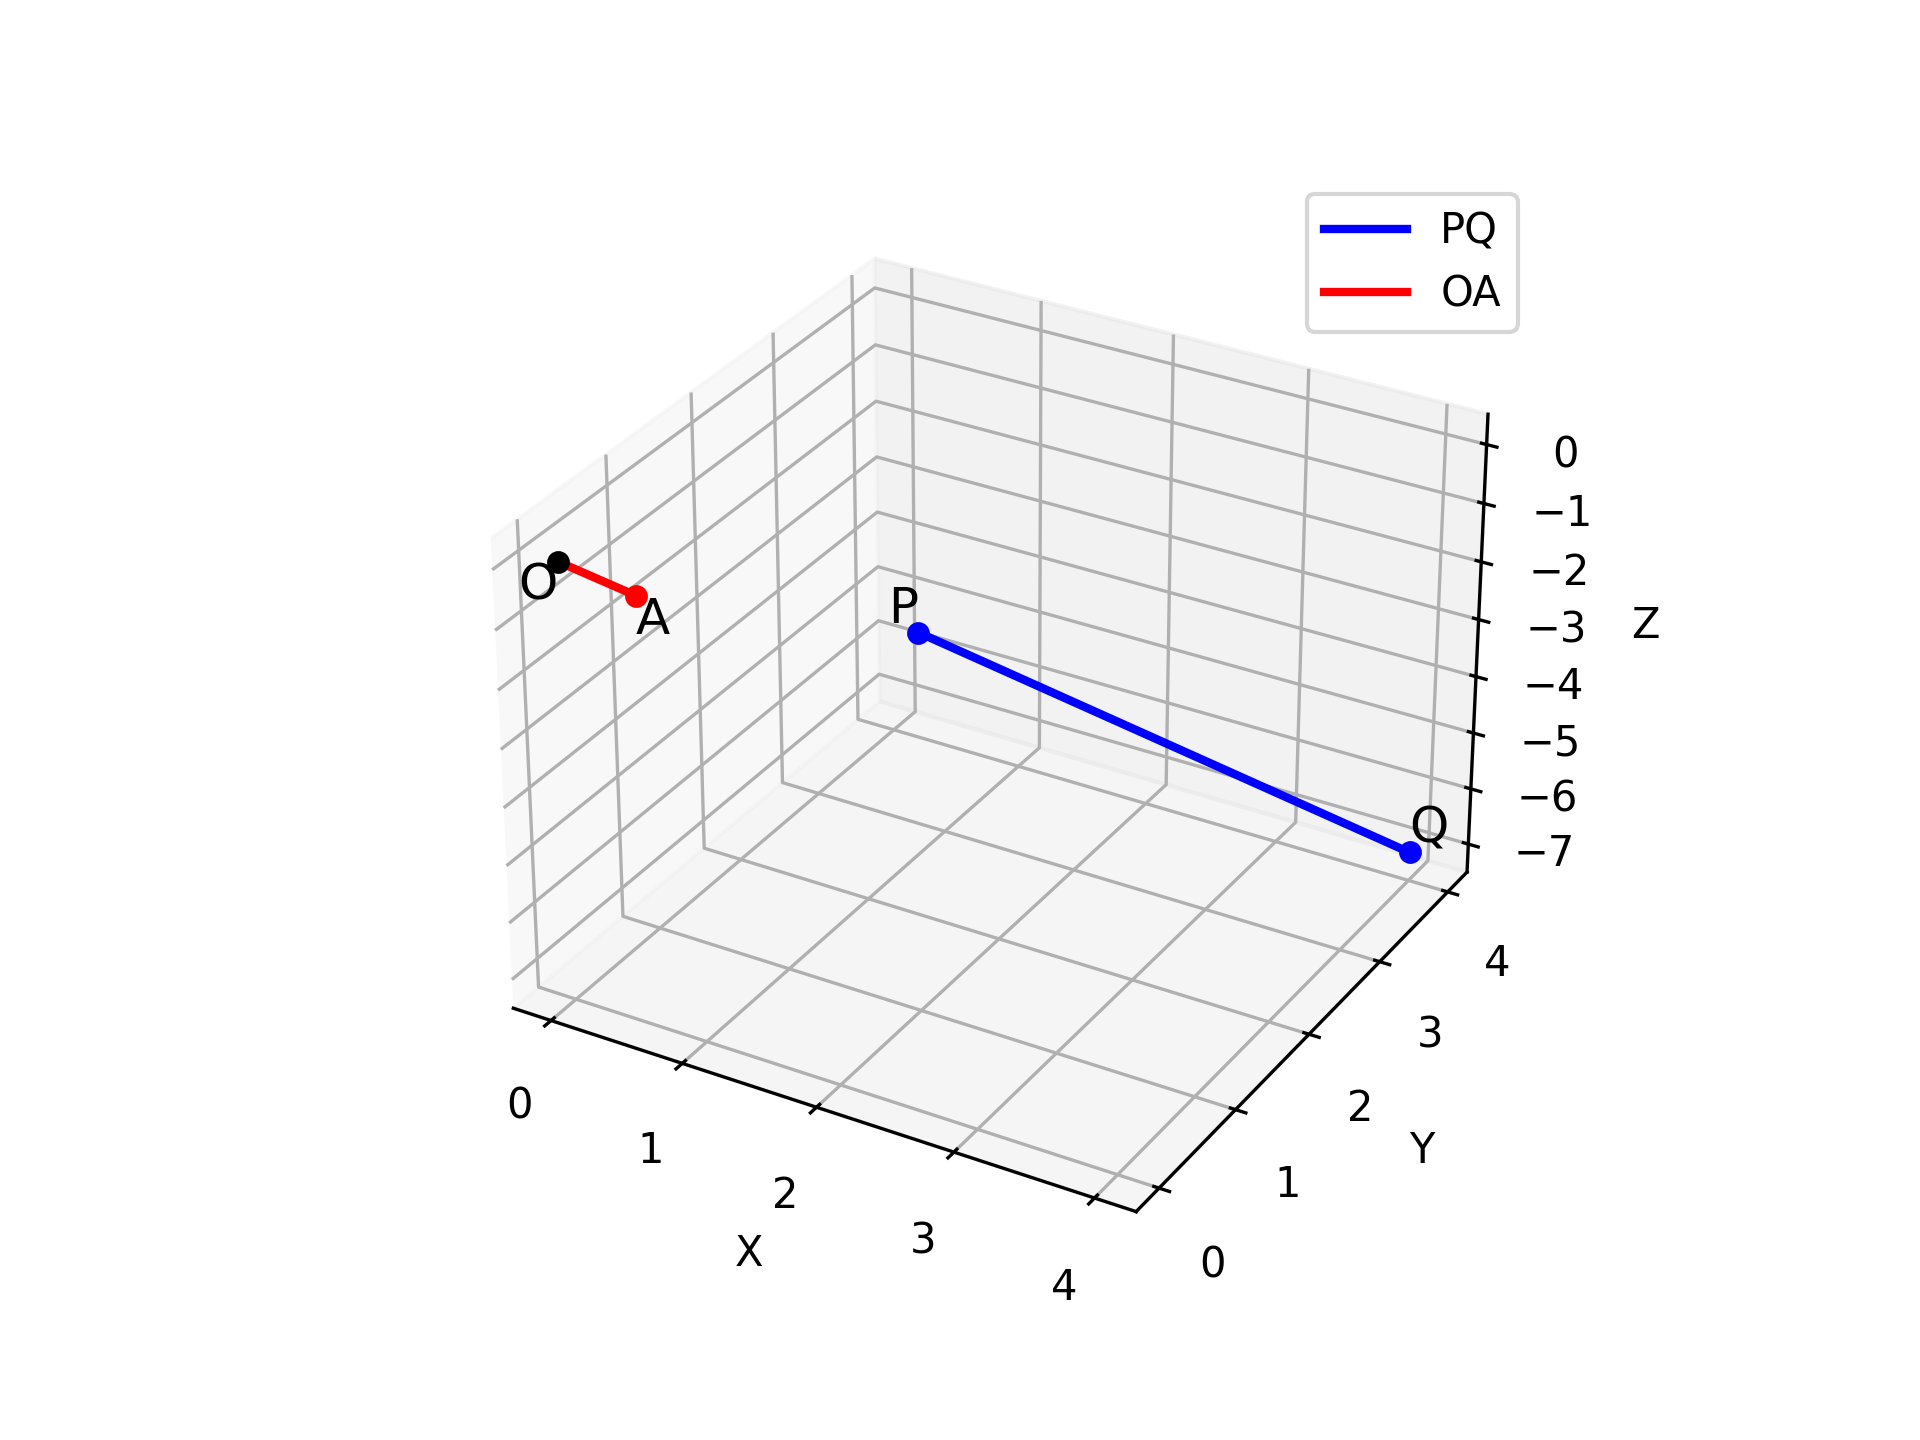
\includegraphics[width=0.6\linewidth]{figs/fig.png}
    \caption{Unit vector $\Vec{OA}$ along $\Vec{PQ}$}
\end{figure}

\end{document}
